\chapter{Implementation}

\change[inline]{TODO: Mention that the location in implementation does 
not use columns, since the presumed location in LibTooling is not
precise.}

The problem analysis in Section~\ref{chap:minimization} established several 
approaches to program reduction and minimization. 
The next step is to compare the described algorithms and techniques. 
Nevertheless, first, we must settle on their concrete implementations. 
More straightforward approaches such as the naive reduction and 
the minimizing Delta debugging algorithm deserve their implementation. 
However, implementing more complicated techniques - static and dynamic 
slicing - is simply out of scope for this project.
This chapter will explain the structure of the project and the implementation 
process of the naive reduction and the minimizing Delta debugging algorithm. 
Moreover, it will introduce the reader to all used technologies and existing 
implementations. 
Each implementation will be described in a high-level overview while 
highlighting the necessary steps for its inclusion in this project. 
The chapter concludes with a discussion on some of the design choices and 
the project's limitations.

\section{Technologies}

This project heavily depends on existing compiler and debugger frameworks. 
Section~\ref{chap:tools} has compared these frameworks and chose the ideal 
candidate for the project. 
That ideal candidate is Clang's LibTooling. 
Section~\ref{chap:libtooling} described in detail the choice of AST as 
the de facto representation of this project's input. 
LibTooling offers multiple ways of traversing and modifying the AST. 
Additionally, it does so for both C and C++.

LibTooling can be built from the LLVM repository together with Clang.
The required versions of Clang (11.0.0) and LibTooling are built from LLVM 
version 11.0.0.
Building LLVM from source is a time-consuming process that does not always 
end in the desired result.
The user must specify all required projects in advance using CMake's options.
LLVM and its projects are then built using a different build tool such as 
ninja or make.
Even though the building process can run multiple jobs at once, it can still 
take up to several hours, consuming a significant amount of the system's 
memory.
The debug build utilizes tens of gigabytes of disk space.
Thankfully, debugging symbols are not required for this project.

Clang is not the only LLVM project required as a prerequisite.
Section~\ref{chap:verification} described the steps of naive validation. 
The final step requires a sort of execution environment. 
One proposed environment is a debugger. 
In order to keep the setup process as simple as possible, we settled on LLDB. 
LLDB is an open-source debugger that ships as a part of the LLVM project.
The user needs to build LLDB with its scripting bridge API.
This can be achieved by adding LLDB to the LLVM project list when invoking 
CMake.
The Python API and its C++ scripting bridge can also be included by 
specifying a few other arguments.
By default, LLVM builds for all available platforms, including ARM and 
PowerPC.
However, only a single platform is required/supported for this project.
The target platform with which LLVM should be built is x86 64 bits.

LibTooling changes with every release.
Projects dependent on an older version of LibTooling might not work with 
a newer one.
Moreover, older releases of LLVM cannot always be built on new platforms.
From experience, the issue might arise when an old LLVM version attempts 
to link new system headers and libraries.
An easy and reliable way of preserving older LibTooling environments is by 
storing them in a Docker container.

Docker is another dependency of this project.
It is required to run slicing implementations as well as support the entire 
minimization process on Windows.

\section{Design}

Since this project compares several techniques, some of which are composed in 
a pipeline, we decided on using a modular design. 
Each reduction approach described in Section~\ref{chap:minimization} consists 
of one or more components. 

These components can be shared and reused across multiple minimizing 
algorithms. 
This choice reduces the amount of copy-pasted code and increases its 
maintainability in the future. 
Depending on the technologies used in each app\-roach, the components form 
either a C++ application or a Python script. 
The latter is required for executing slicer implementations. 
This fact leads to inconsistent interface across multiple reduction 
approaches. 
For example, the user can launch the minimizing Delta debugging algorithm as 
a C++ console application. 
However, if he decides to execute the slicing-based approach, he will need 
to launch it as a Python script.

\begin{figure}[h]\centering
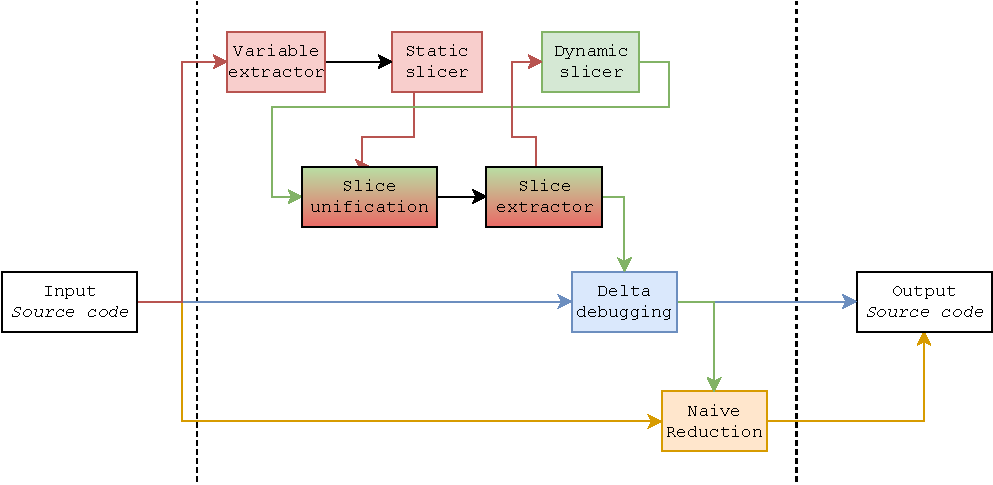
\includegraphics[scale=0.85]{components}
\caption{Communication between modules in three different pipelines:
Naive (orange), Delta (blue), Slicing (red and green).}
\label{img:components}
\end{figure}

Figure~\ref{img:components} shows a diagram of all available pipelines and 
their shared modules. 
Since some pipelines only add a preprocessing layer, they end up reusing 
the fundamental components of simpler pipelines.
Each module shown in the diagram will be described in the following sections.

\section{External code}

Some of the external code cannot be added to the C++ project due to 
compatibility reasons.

Giri\change[]{TODO: Read the notes and the over\-view, summarize the contents.}

DG\change[]{TODO: Read the notes and the over\-view, summarize the contents.}

\section{Shared components}

As was already mentioned, this project reuses several ideas and components 
in multiple approaches. 
One component does not necessarily translate to one idea. 
It often takes a couple of modules to capture that idea. 
The following subsections will describe each idea proposed in previous 
chapters. 
Each subsection will then outline components used by its particular idea.

\subsection*{Recursive visitor}

Some of the ideas in the following sections require us to traverse and alter 
the AST.
As explained in Section~\ref{chap:ast}, LibTooling allows us to traverse 
the AST using two methods. 
Splitting the code into code units could be done with either 
the \icode{RecursiveASTVisitor} or \icode{ASTMatchers}. 
We chose to implement the visitor interface to preserve more consistency 
across the project. 
Using a LibTooling visitor requires implementing three classes. 
Types of their implementation are described in detail in the following 
paragraphs.

\paragraph{Actions.} Each derivation of \icode{ASTFrontendAction} can have 
its own preprocessing and postprocessing steps.
Other than performing an action before and after a file is handled, it also 
creates a specific visitor.
In this project, we only utilize \icode{ASTFrontendAction} to create 
a consumer.
Moreover, the usage of actions tends to be module-specific. 
Usually, each component has its \emph{Actions.cpp} and \emph{Actions.h} files.
Further, some of the derivations use their custom factories.
By default, any \icode{ASTFrontendAction} can be created by calling 
the \icode{FrontendActionFactory::create()} method.
The method uses the default constructor and thus cannot provide any 
arguments for concrete \icode{ASTFrontendAction} implementations.
A workaround can be seen in \emph{Actions.cpp} files, most of which contain 
a custom factory.
The factory takes the necessary parameters, calls the desired constructor,
and passes them to a \icode{Consumer} instance in its \icode{create()} method.

\paragraph{Consumers.} This project distinguishes two types of 
\icode{Consumer} implementations. 
The first is a module-specific type. 
These \icode{Consumer} implementations contain high-level actions of 
a specific algorithm and are used for data transfer. 
For example, the \icode{VariantGeneratingConsumer} does not invoke any 
visitor instances. 
Instead, it keeps references to two more granular \icode{Consumer} objects. 
The \icode{VariantGeneratingConsumer} contains the main loop of the naive 
algorithm shown in Figure~\ref{chap:naive}. 
The pair of more granular consumers then carries out specific actions. 
The module-specific consumer also handles data exchanges between its more 
specific workers. 
One way of doing these exchanges is by keeping data structure instances 
inside the parent consumer. 
Another is by accessing the worker's internal states, either through their 
fields or getter methods. 
In summary, the module-specific consumer's job is to organize the granular 
parts of an algorithm, execute their actions, and collect their results.

The second \icode{Consumer} type is the shared consumer. 
These consumers are used for dispatching shared visitors, reporting their 
state, and collecting their data. 
The shared consumer responsible for code unit separation is 
the \icode{Dependency\-Mapping\-AST\-Consumer}. 
It dispatches a concrete visitor to the top-most node and offers getter 
methods to retrieve the visitor's data. 
This consumer also contains some logic in its 
\icode{HandleTranslationUnit} method. 
Other than dispatching the visitor, it also saves a visualization of 
the current AST. 
Other shared consumers might contain different logic in that method.


\paragraph{Visitors.} Visitors are once again separated into two types. 
A specific algorithm might use its unique visitor implementation to do 
an action such as slice extraction. 
This type of visitor is tied to a corresponding module-specific consumer. 
Similarly, shared visitors are also bound to their corresponding shared 
consumers. 
However, shared visitors are used for tasks that are used in both the naive 
and Delta algorithms. 
Those tasks are the node mapping and the variant generation. 
In our case, visitors contain the logic of a single iteration. 
Be it an iteration of the naive minimization or the Delta debugging; 
visitors are dispatched polynomially or even exponentially many times. 
The logic generally contains rules for handling each type of language 
construct. 
Two examples of such rules are:
\begin{itemize}
  \item Skipping the traversal of an implicit cast node of type 
  \icode{ImplicitCastExpr}, since removing it will not alter the source code.
  \item Creating a code unit for each statement that is not an expression.
\end{itemize}
The logic of a shared visitor is reused in multiple projects. 
This logic might include splitting the source code into code units. 
A module-specific visitor's logic is oriented to a particular problem, 
such as scanning the locations of statements in the code.

\subsection*{Code units}

Initially, a code unit was defined as any syntactically correct subset of 
the source code. 
It was then narrowed down to an atomic code unit - the smallest sensible 
syntactically correct source code element. 
Both the naive and the Delta algorithms use code units to perform their 
reductions. 
The goal is to split a given source code into partitions that can be later 
kept or removed. 
Those partitions would ideally not overlap and could be therefore 
independently removed.

We can split the input source code into code units by traversing its AST 
with a specified granularity. 
The idea is to analyze nodes based on hand-written rules. 
These rules specify which nodes are worth visiting and how to process them. 
While we are partitioning the source code, we might as well map the code's 
dependencies. 
This mapping can be done by extending our rules to perform specific lookup 
operations during the traversal. 
For example, the algorithm looks up all variable usages for a given variable 
declaration node. 
The results of those lookups are then kept in the dependency graph described 
in Section~\ref{chap:heuristics}.

\paragraph{Consumers.} The single consumer dedicated to code unit separation 
is implemented in the \icode{DependencyMappingASTConsumer} class. 
The consumer serves as a middle man for data transfers. 
Notably, it can retrieve data for the following structures:
\begin{itemize}
  \item Node mapping - this mapping is a lookup table that transitions 
  between a node's internal ID given by Clang and the current traversal 
  order number. 
  The traversal order number specifies the order in which the current node 
  is visited once the visitor is dispatched using 
  \icode{HandleTranslationUnit}. 
  The mapping is later transferred to other visitors to achieve the same 
  traversal order.
  \item Code units count - this property returns the total amount of code 
  units once their partitioning is complete.
  \item Dependency graph - is represented by a directional graph of nodes, 
  where each node is represented using its traversal order number. 
  Nodes in the graph might also contain additional information used for 
  debugging, such as their type and the code snippet they represent.
  \item Skipped nodes - this container serves as a list of nodes not worth 
  visiting. 
  These nodes might be too granular or solely implicit.
\end{itemize}
The consumer dispatches its concrete visitor, which carries most of 
the logic. 
The only standalone logic in the consumer is to dump a visualization of 
the source code based on the dependency graph.

\paragraph{Visitors.} What becomes a code unit is decided inside 
the \icode{MappingASTVisitor} class. 
The visitor traverses the AST in a postorder manner and stops at specified 
declarations, statements, and expressions. 
Each of these nodes must fulfill a predicate - their specific rule - to 
become a code unit. 
The node must not be a duplicate of an already visited node. 
It must also be a part of the main source file, i.e., not a part of a system 
header file. 
If the node satisfies all three requirements, it is considered a code unit. 
The node's ID mapping is then created, and the node is added to 
the dependency graph. 
On the other hand, if the node is not a valid code unit, it is added to 
the skipped nodes list. 
In that case, the next visitor will not consider visiting and manipulating 
the node when traversing the AST.

\subsection*{Bitfield to variant transformation}

Once the number of code units is known, we can create a bitfield of that 
size and generate representations of possible variants. 
The mechanism of generating bitfields was explained in 
Section~\ref{chap:naive}. 
This section describes the necessary parts of a technique that converts 
bitfields into source code variants. 
The idea is to flag AST nodes as code units and then traverse the AST again, 
removing the code unit nodes specified by a given bitfield. 
A single iteration of the variant-generating techniques produces one source 
code variant. 
The variant is created by starting with the original source code and 
gradually removing nodes. 
Each node has its index in the given bitfield. 
The index corresponds to the node's traversal order number. 
A node is removed if its corresponding bit is set to zero. 
To be more precise: the node is not removed from the AST. 
Instead, only its underlying source code is removed. 
The following paragraphs describe the code behind the removal.

\paragraph{Consumers.} All the necessary data for bitfield to source code 
conversion is acquired using the \icode{VariantPrintingASTConsumer}. 
This consumer dispatches its specific visitor and provides it with 
a bitfield. 
The visitor then removes snippets of the code based on that bitfield.
The consumer's job is to reset the visitor's state, launch it with 
the provided bitfield, and save its output into a specified file. 
The consumer can also access the visitor's internal state, namely its 
adjusted error line location. 
More details about this location can be found in the \emph{Visitors} section.

\paragraph{Visitors.} Similar to the code unit mapping issue, 
the \icode{Variant\-Printing\-AST\-Visitor} carries most of the conversion's 
logic.
It is provided with a bitfield, which it saves, and a \icode{Rewriter} 
instance, which it uses to generate the variant.
Section~\ref{chap:sts} describes the \icode{Rewriter} class in more detail.
Traversal of the source code is done in a postorder fashion to stay 
consistent with the previous visitor. 
The previous visitor shares its dependency graph and its list of skipped 
nodes.
This way, the \icode{VariantPrintingASTVisitor} can traverse the AST the way 
it was intended to. 

Each code unit, i.e., visited node, is removed if it fulfills specific 
requirements. 
First, the node's bit must be set to zero. 
Second, all its parent's bits must be set to one. 
The latter is a \icode{Rewriter} requirement. 
A parent node might represent a compound statement, and its children might 
be the individual statements inside the parent. 
If we were to remove the parent and one of its children, we would remove 
the same snippet twice. 
This catch would eventually lead to an error. 
The error can be avoided by only removing children while keeping their 
parents.
Once the AST traversal is done, all unwanted code units are removed. 
We are left with a \icode{Rewriter} instance whose buffer reflects 
the current variant. 
The visitor's iteration is done, and it is the consumer's job to save 
the contents of the buffer.

\subsection*{Variant validation}

Testing results on whether they are valid variants requires a standard 
interface, too.
Section~\ref{chap:verification} describes the steps in the process 
of validation.
The implementation contains three parts that are used in all approaches 
presented in this project.
Below is the description of compilation, analysis, and execution.

\paragraph{Compilation.} By calling the \icode{Compile} function in 
\emph{Helper.cpp}, one can invoke the Clang compiler driver.
The compiler has two goals.
Firstly, it filters out non-compilable and thus invalid variants.
Secondly, it prepares compilable variants for the execution stage.
The compilation can be invoked with a wide range of arguments.
In this case, it is provided with the \icode{-g} and \icode{-O0} options.
The former generates debug symbols for the executable, while the latter 
ensures reliable debugging by eliminating any compiler optimizations.
Compilation's output is printed to the standard output, and its exit status 
determines the function's return value.
If the compiler terminates with a valid exit code but does not create 
the binary, the function returns as if the compilation failed.
The binary is stored to a specified path, which by default is the same file 
path as the input source file.
The file extension is substituted with \icode{.exe}.

\paragraph{Static analysis.}
\change[inline]{TODO: Research and implement calls to the Clang static analyzer.}

\paragraph{Execution.} Compiled binaries need to be validated at runtime.
This way, we check whether the program results in the desired runtime error.
Programs are executed in the LLDB environment.
LLDB provides Python API, which allows invoking more or less all of 
the debugger's commands.
The API is also available from C++ using a scripting bridge.
SWIG processes function calls made from C++.
They then produce bindings to the Python API.
Thanks to the scripting bridge, every validation step is written in C++.
The \icode{ValidateResults} function creates a debugging environment for every 
executable.

The programs are then run in separate processes.
During the execution, events are broadcasted from the forked processes.
The stack trace is investigated whenever the program broadcasts a stopped 
state, indicating a thrown exception.
If the symbol's location on top of the stack trace is the same as the one of 
the desired error, the program is tagged as valid.
Otherwise, the execution continues.

\section{Naive reduction}

The algorithm for naive minimization is the foundation of this project. 
The approach and its heuristics were described in detail in 
Section~\ref{chap:naive}. 
The naive algorithm can guarantee minimality. 
Unfortunately, the same cannot be said for greedy approaches. 
Since this project focuses heavily on minimization, we dedicated 
a significant amount of time to improving the naive approach's implementation.

The approach works by deploying a \icode{DependencyMappingConsumer}, whose 
primary job is to split the AST into code units.
The mentioned consumer dispatches a visitor that creates the traversal order.
The visitor considers declarations and statements.
It determines whether these nodes should be visited by the other visitors and 
maps their dependencies.
In short, one node is dependent on another if it is in the other node's 
subtree.
Another rule for node dependencies states that usages of variables depend on 
their declarations.
Function definitions and calls follow a similar rule.

Once the \icode{MappingASTVisitor} has traversed the AST, 
the \icode{Dependency\-Map\-ping\-Consumer} collects its output, and the 
variant generating function is initialized.
Before any actual variants are created, the algorithm first separates all 
valid variants into bins of different sizes—the binning works as follows.
The \icode{Dependency\-Mapping\-Consumer} has determined $n$: the number of 
code units in the file.
Moreover, it has set the order in which nodes are traversed.

We can create a bitfield of size $n$, where the $i^{th}$ bit represents 
the $i^{th}$ node in the traversal order.
If the bit is set to \icode{true}, the node will be preserved.
Otherwise, it will be removed from the variant.
This gives us $2^n$ bitfield variants, the same number required for all 
program variants.
With the bitfield representation, we could use bitwise operations to move 
between different variants.
The only operation necessary for generating all variants is the increment 
function.
While cycling through all possible bitfield configurations, we check that 
each obeys the dependency rules.
Valid bitfields also carry the source code size of the program variant they 
represent.
Variants are assigned into categories based on their represented size.

The idea is to search iteratively, generate minor source code variants, and 
validate them first before moving on to the remaining possible variants.
The number of bins represents the granularity with which the deepening 
search is conducted.
It makes sense to set the granularity high for more extensive programs.
After the binning process is complete, the variant generating loop is 
launched.

The loop considers all bitfields in a given bin.
In each iteration, the bitfield is passed to 
a \icode{VariantPrintingASTVisitor}.
The visitor traverses the AST in the order given by 
the \icode{MappingASTVisitor}.
The nodes represented by the bitfield are either kept or removed based on 
the value of each bit.
It should be stated that the nodes are not removed.
Instead, it is the underlying source code that is being deleted using 
a \icode{Rewriter} operation.
The removal also follows an explicit rule.
Nodes are removed only if their parents will not be removed.
This rule eliminates the chance of removing an underlying code snippet twice.
Each \icode{VariantPrintingASTVisitor} handles a single variant.

After all variants from the given bit are processed, all results are tested 
for validation.
In case a valid result is found, the search ends.
Otherwise, the search continues with the bin representing the following 
smallest variant sizes.

\section{Delta debugging}

\section{Systematic approach}

\change[inline]{TODO: Might require mentioning the component that unifies slices or extracts all variables from a line.}

The systematic approach comprises multiple steps.
The motivation behind these steps and an overview of the algorithm can be 
found in section~\ref{chap:systematic}.

This approach uses external code that cannot be trivially added to 
the project.
Therefore, it is launched and operated differently.
The base is a Python script that invokes all necessary components.
The script uses Docker API to launch a DG container.
It also maps input and output directories to that container in order to send 
and retrieve data.
The container's launch command invokes the slicer to process the given input 
and store it in the given output directory.
Giri is launched analogically.

Both slicers return a list of lines that represent the slices.
This output needs to be processed further.
The script invokes the \icode{SliceExtractor} program.
The program transforms a source file into the desired slice based on 
the given list of lines.
It does so based on ASTMatchers, removing the complement of the given list 
of lines by using \icode{Rewriter} operations.
Once the \icode{SliceExtractor} produces the desired source file, the file 
is considered the respective slicer's output.
This way, each step of the algorithm results in a valid source file.

After passing through the two slicers, the intermediate result is further 
reduced using the naive approach.
The Python script executes the naive algorithm, which then produces the 
desired results.
Another approach can also substitute the ultimate step.
One can easily swap between the naive reduction and Delta debugging by 
simply changing the path to the executable in the Python script.